\documentclass{beamer}

\usepackage[utf8]{inputenc}
\usepackage[T1]{fontenc}
\usepackage{amsmath}
\usepackage{bm}

\usepackage{tabularx}
\usepackage{graphicx}
\usepackage{epstopdf}
\usepackage{multirow}

\graphicspath{{../../images/}}

\usetheme{Madrid}
\usebeamercolor{sidebartab}
\usefonttheme{professionalfonts}


\title[M.Sc. Thesis 2015]{Spatial Summarization of Image Collections}
\author{Diego A. Ballesteros Villamizar}
\institute[ETHZ]{ETH Zürich}
\date{February 29th, 2016}

\DeclareMathOperator*{\argmin}{argmin}
\DeclareMathOperator*{\argmax}{argmax}

\AtBeginSection[]
{
  \begin{frame}<beamer>
    \frametitle{Outline}
    \tableofcontents[currentsection]
  \end{frame}
}

\begin{document}

\begin{frame}
  \titlepage
\end{frame}

\section{Featurized Model}

\begin{frame}{Gaussian features}
  \begin{itemize}
    \item Features matrix
    \begin{align*}
    \mathbf{X} \in \mathbb{R}^{|V| \times |V|} \\
    x_{ij} = \exp{\left(-\frac{\left({lat}_{j} - {lat}_{i}\right)^2 + \left({lon}_{j} - {lon}_{i}\right)^2}{2 \sigma^{2}}\right)}
    \end{align*}
    \item For $\sigma = 0$, $\mathbf{X} = \mathbb{I}$.
    \item Latitudes and longitudes are scaled to [0,1] on the set of items.
  \end{itemize}
\end{frame}

\begin{frame}{$\sigma$ effect}
  \begin{figure}
    \centering
    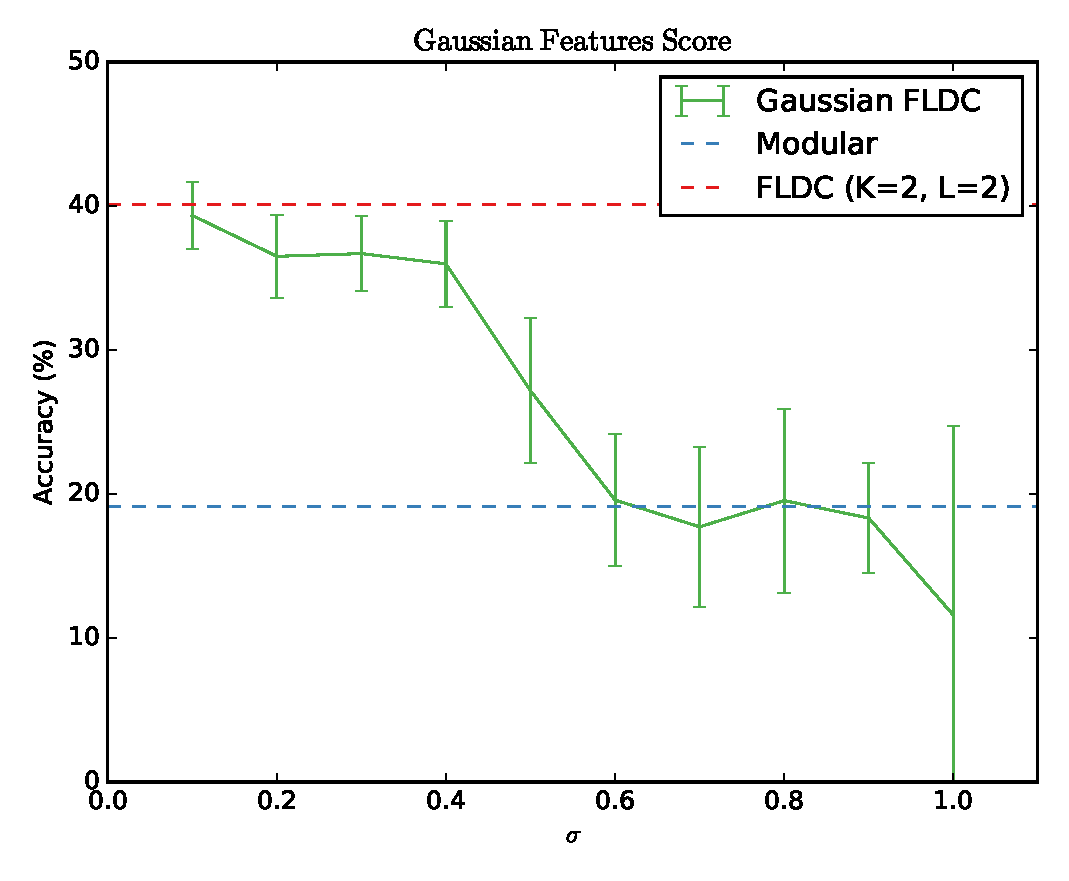
\includegraphics[height=0.8\textheight]{gaussian_features_score}
  \end{figure}
\end{frame}

\begin{frame}{Effect number of features}
  \begin{figure}
    \centering
    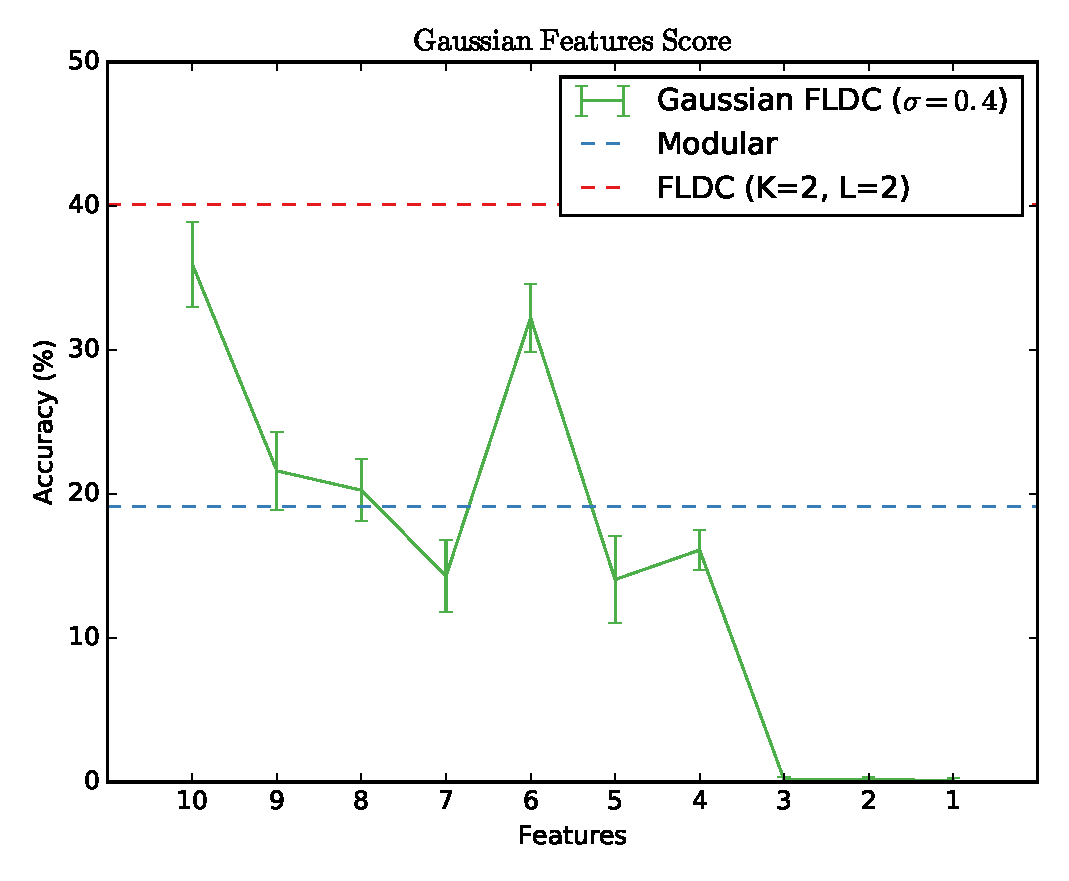
\includegraphics[height=0.8\textheight]{gaussian_features_score_size}
  \end{figure}
\end{frame}

\section{Synthetic Datasets}

\begin{frame}{One-dimension model}
  \begin{itemize}
    \item FLID model with 3 items.
    \begin{align*}
      \mathbf{u} &= [2,1,1] \\
      \mathbf{W} &= [0,100,100]^\intercal
    \end{align*}
    \item Distribution is:
      \begin{itemize}
        \item \{0\}: 13.94\%
        \item \{1\}, \{2\}: 5.13\%
        \item \{0,1\}, \{0,2\}: 37.90\%
        \item \{1,2\}, \{0,1,2\}: 0.00\%
      \end{itemize}
  \end{itemize}
\end{frame}

\begin{frame}{Learning accuracy}
  \begin{itemize}
    \item Dataset generated with 10k samples.
    \item Modular and FLID model trained on this dataset.
    \item When conditioning on 1 or 2, both models get the prediction right.
    \item When conditioning on 0, there is no information. Both 1 and 2 are equally likely, only in half of the cases the models get it right.
  \end{itemize}
  \begin{table}
    \centering
    \begin{tabular}{@{}ll@{}}
      \hline
      \textbf{Model} & \textbf{Accuracy (\%)}\\
      \hline
      Modular & $75.23 \pm 0.82$ \\
      FLID (L=1) & $74.96 \pm 2.04$ \\
      \hline
    \end{tabular}
  \end{table}
\end{frame}

\begin{frame}{Learned distribution}
  \begin{itemize}
    \item Scores are equal but learned distributions are different.
    \item For modular (one of the folds):
      \begin{itemize}
        \item \{0\}: 30.17\%
        \item \{1\}, \{2\}: 2.64\%, 2.74\%
        \item \{0,1\}, \{0,2\}: 22.26\%, 23.11\%
        \item \{1,2\}, \{0,1,2\}: 2.02\%, 17.05\%
      \end{itemize}
    \item For FLID (one of the folds):
      \begin{itemize}
        \item \{0\}: 16.07\%
        \item \{1\}, \{2\}: 5.59\%, 5.17\%
        \item \{0,1\}, \{0,2\}: 37.36\%, 34.59\%
        \item \{1,2\}, \{0,1,2\}: 0.16\%, 1.07\%
      \end{itemize}
    \item Learned FLID model (one of the folds):
      \begin{align*}
        \mathbf{u} &= [1.92, 0.87, 0.79] \\
        \mathbf{W} &= [0.02, 4.34, 4.34]^\intercal
      \end{align*}
  \end{itemize}
\end{frame}

\begin{frame}{FLDC dataset}
  \begin{itemize}
    \item FLDC model with 4 items.
    \begin{align*}
    \mathbf{u} &= [1,1,1,1] \\
    \mathbf{W}_{D} &= \left( \begin{array}{cccc}
    100 & 100 & 0 & 0 \\
    0 & 0 & 100 & 100 \\
    100 & 0 & 100 & 0 \\
    0 & 100 & 0 & 100 \end{array} \right) \\
    \mathbf{W}_{C} &= \left( \begin{array}{cc}
    5 & 0 \\
    5 & 0  \\
    0 & 5 \\
    0 & 5 \end{array} \right)
    \end{align*}
    \item Distribution is:
    \begin{itemize}
      \item \{0\}, \{1\}, \{2\}, \{3\}: 10.60\%
      \item \{0,1\}, \{2,3\}: 28.81\%
      \item \{0,2\}, \{0,3\}, \dots: 0.00\%
      \item \{0,1,2\}, \{0,1,3\}, \dots: 0.00\%
    \end{itemize}
  \end{itemize}
\end{frame}

\begin{frame}{Learning accuracy}
  \begin{table}
    \centering
    \begin{tabular}{@{}ll@{}}
      \hline
      \textbf{Model} & \textbf{Accuracy (\%)}\\
      \hline
      Modular & $50.61 \pm 1.72$ \\
      FLID (L=1) & $49.39 \pm 1.72$ \\
      FLID (L=2) & $69.37 \pm 25.02$ \\
      FLID (L=3) & $79.54 \pm 25.10$ \\
      FLID (L=4) & $84.79 \pm 23.25$ \\
      FLDC (L=4, K=2) & $100.0 \pm 0.00$ \\
      \hline
    \end{tabular}
  \end{table}
\end{frame}

\begin{frame}{Learning method problems}
  \begin{itemize}
    \item 2 dimensions are enough to achieve 100\% accuracy. But only a few of the folds learn properly.
    \item As the number of parameters increases, it's more likely that all folds will learn correctly.
    \item A good $L=2$ model is:
      \begin{align*}
      \mathbf{u} &= [0.18,7.46,3.68,3.69] \\
      \mathbf{W}_{D} &= \left( \begin{array}{cc}
      0.02 & 0.02 \\
      8.46 & 8.47 \\
      8.46 & 0.02 \\
      0.02 & 8.47 \end{array} \right)
      \end{align*}
  \end{itemize}
\end{frame}

\begin{frame}{Learned model}
  \begin{itemize}
    \item For the same number of parameters as the original model.
    \item The learned FLDC model for $L=4$ and $K=2$ is:
      \begin{align*}
      \mathbf{u} &= [0.01,-0.16,1.89,1.89] \\
      \mathbf{W}_{D} &= \left( \begin{array}{cccc}
      5.25 & 5.25 & 0.05 & 0.05 \\
      0.039 & 0.039 & 5.22 & 5.22 \\
      5.25 & 0.034 & 0.034 & 5.22 \\
      0.035 & 5.25 & 5.22 & 0.035 \end{array} \right) \\
      \mathbf{W}_{C} &= \left( \begin{array}{cc}
      3.48 & 3.48 \\
      3.50 & 3.50  \\
      1.39 & 1.36 \\
      1.36 & 1.39 \end{array} \right)
      \end{align*}
  \end{itemize}
\end{frame}

%\begin{frame}{References}
%  \bibliographystyle{acm}
%  \bibliography{../references}
%\end{frame}

\end{document}
